\documentclass{IOS-Book-Article}
\usepackage[T1]{fontenc}
\usepackage[utf8]{inputenc}
\usepackage{graphicx}
\usepackage{mathptmx}
\usepackage{paralist}
\usepackage{epstopdf}
\usepackage{paralist}
\usepackage{tikz}
\usepackage{ctable}
\usepackage{caption,subcaption}
\usepackage{csquotes}
\usepackage{mathtools}
\usepackage[numbers]{natbib}
%\bibliographystyle{dcu}
\bibliographystyle{unsrtnat}
\setlength{\marginparwidth}{4cm}
\usepackage[textsize=tiny]{todonotes}
\usepackage{url}
\def\hb{\hbox to 10.7 cm{}}

\newcommand{\dara}{\textsf{da\textbar ra}}
\begin{document}

\pagestyle{headings}
\def\thepage{}

\begin{frontmatter}
\title{A Semi-Automatic Approach for Improving Dataset References in Social Sciences Full Texts}

\author[A,B]{\fnms{Behnam} \snm{Ghavimi}
\thanks{E-mail: Behnam.Ghavimi@gesis.org}},
\author[A]{\fnms{Philipp} \snm{Mayr}
\thanks{E-mail: Philipp.Mayr@gesis.org}},
\author[B]{\fnms{Sahar} \snm{Vahdati}
+\thanks{E-mail: vahdati@cs.uni-bonn.de}}
and
\author[B,C]{\fnms{Christoph} \snm{Lange} 
\thanks{E-mail: langec@cs.uni-bonn.de}}

\address[A]{GESIS – Leibniz Institute for the Social Sciences}
+\address[B]{Enterprise Information Systems (EIS), University of Bonn}
+\address[C]{Fraunhofer Institute for Intelligent Analysis and Information Systems IAIS}
\begin{abstract}
\todo[inline]{SV@BG: usually negative start is not the best way to start, I suggest that you turn the sentence in a positive one and add one introductory sentence also, you are too quick to say what is there and what we lack. I did some changes already.\\ CL: I changed some more; in any case the negative start is not \emph{that} problematic for me.}
Today, full texts of scientific papers are often stored in different places than their underlying research datasets.
%<newpart_0
As a first step towards a closer integration, there now exist several online registries that make datasets citable – but current authoring lack integration of such repositories. 
%newpart_0>
As a consequence, explicit links to datasets are generally missing in papers; authors refer to datasets using title and year of publication.
\todo[inline]{CL: The following is a new and IMHO important point.}It is thus hard to reproduce the authors' results, to access the datasets underlying papers for further analysis, and to determine the impact of a dataset.
Manually detecting references to datasets in scientific papers is a time-consuming task and requires expert knowledge in the underlying research domain. 
We propose and evaluate a semi-automatic approach for finding explicit references to datasets in social sciences papers.

%<newpart_1
Our approach comprises three main steps: extracting pre-defined special features from datasets' titles in the {\dara} registry, detecting references to datasets using the extracted features, and matching the references found with corresponding datasets' titles.
%newpart_1> 
The approach does not require a corpus of papers (no cold start problem) \todo[inline]{SV@BG:I do not understand this\\ CL: the “cold start problem” thing is sufficiently clear to me}and it performs well on a small test corpus (\todo[inline]{CL@BG: This phrasing suggests that “test corpus” and “gold standard” are the same.  But the way I understand “corpus” in the context of our problem is that it's a set of documents (i.e.\ input to our algorithm), whereas a “gold standard” should be something like a set of documents plus their links to datasets (i.e.\ input plus expected output).}gold standard). 
Our approach achieved an F-measure of 0.84 for detecting references in full texts and an F-measure of 0.83 for finding correct matches of detected references in the {\dara} dataset registry. \todo[inline]{SV@BG:I would not give exact figures here, tell a general results, what we have achieved\\ CL: I disagree.  I checked previous IS\&U abstracts, and it's not entirely uncommon to be that precise in the abstract.}
\todo[inline, size=\tiny]{Abstract should not be more that 200 words - Currently. It is 183 words. }
\end{abstract}

\begin{keyword}
Information extraction\sep Link discovery\sep Data linking\sep Research data\sep Social Sciences\sep Scientific papers
\end{keyword}
\end{frontmatter}
\section{Introduction}
Digital libraries have been growing enormously in recent years. \todo{SV@BG:try to have sentences that carry some value, this is not good to start the intro with such sentence, align it with abstract, even use the same sentence and expand each sentence of the abstract as one paragraph in intro}
Digital libraries aim at providing resources with high metadata quality, easy subject access, and support for retrieving information~\citep{Hienert2015}. 
% We are specifically interested in scientific full text papers in digital libraries.\todo[inline, size=\tiny]{SV@BG:saying we are interested on sth is not scientific at all, rephrase it and include the reason.\\ CL: This sentence is not necessary to introduce our point, so I've commented it out.}
Today, in the quantitative social sciences and other fields, many papers make references to research datasets on which they are based, in that they, e.g., present the results of a statistical analysis over some dataset.
However, these references are usually not explicitly exposed in digital libraries.
In most cases the papers do not provide explicit links that would give readers direct access to the referenced datasets. 

Explicit links from scientific publications to the underlying datasets and vice versa can be useful in multiple use cases, including the following:
\begin{itemize}
	\item reviewers exploring to reproduce the evaluation that a paper's authors performed on a dataset, 
	%a link would give him straightforward access to the data, enabling them to check the evaluation,
	\item other researchers desiring to perform further analysis on a dataset that was used in a paper,
        \item decision makers seeking to determine the impact of a given dataset (by counting its citations) or to identify the most important datasets in a given community.
\end{itemize}% \todo[inline, size=\tiny]{SV@BG:add two more use cases\\ CL: I added some.} 

Currently, the majority of published papers lacks such direct links to datasets.
\todo{SV@BG:add one more sentence about the state of current papers, how they do refer to datasets\\ CL: I think this is sufficiently covered below.}
While there exist registries that make datasets citable, e.g., by assigning a digital object identifier (DOI) to them, they are usually not integrated with authoring tools.
Therefore, in practice, authors typically cite datasets by \emph{mentioning} them, e.g., using  
combinations of title, abbreviation and year of publication (see, e.g., \citet{Mathiak2015}).  

Manually detecting references to datasets in papers is time consuming and requires expert knowledge of the paper's domain. 
Detecting dataset references automatically is challenging since \todo{CL@BG: to provide evidence for the following claim, please cite something suitable.}in most cases, approaches need a huge corpus of papers as training set. 

%<newpart_2
It is a difficult task to create such a training set manually due to the wide variety of styles of dataset citations in full texts even within one research community, and the multitude of \todo{CL@BG: Is the following what you meant by “stored places for dataset citation”?  If so, I tried to phrase it more clearly.}places in papers in which such citations can occur (illustrated by Figure~\ref{fig:places-example}).
%newpart_2>

\begin{figure}[h]
	\centering
	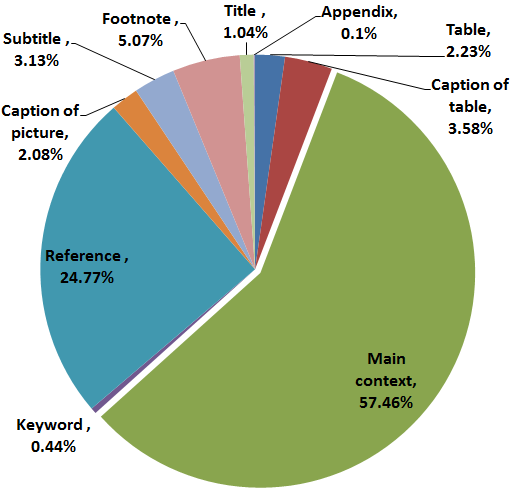
\includegraphics[width=3.5in]{DistPlaces3.PNG} \todo[inline, size=\tiny]{SV@BG: bad quality, recheck the figure\\ CL: export the figure in a vector format or, if only bitmap is possible, with a higher resolution.}
	\caption{The distribution of dataset references in 15 random papers from the mda journal (see Section~\ref{sec:mda})}
	\label{fig:places-example}
\end{figure}

%<newpart_3
This variance even makes rule-based approaches difficult, as it is hard to cover all cases. \todo{SV@BG:give 1-2 concrete technical reasons why it makes it difficult\\ CL: Indeed: 1–2 examples of extreme but still common cases of “this variance”, please.}
\todo{CL@BG: I tried to phrase the following a bit more precisely, but still a concrete reference would be good.}Approaches that learn from a corpus of papers require large amounts of disk space and processing time.
%newpart_3>
We therefore introduce a semi-automatic approach to solve this problem that parses full texts with high performance and finds exact matches with a high precision, without requiring a training set. 
In the remainder of this section\dots \todo{SV@BG:say what is going to come in subsections} 

\subsection{Problem Statement}
Whereas a lot of effort has been spent on information extraction in general~\citep{Sarawagi2007}, few attempts have focused on the specific use case of dataset extraction (see, e.g., \citep{MeiyuLu2012}). \todo{SV@BG:effort on information extraction and dataset extraction is not comparable, one is a research field, the other is a usecase, rephrase it.\\ CL: I made the first step: not yet perfect, but better.}
When referring to the same dataset, different authors often use different names or keywords.
Although there are proposed standards for dataset citation in full texts, researchers still ignore or neglect such standards.
One of the important standards is proposed by~\citeauthor{altman2007proposed} for dataset citation~\citeyearpar{altman2007proposed}.
\todo{SV@BG:say a bit about this standard\\ CL: Yes, please – or, if you can't, shorten this sentence to “see, e.g., \cite{altman2007proposed}” and merge it into the previous one.}
Since the structure of scientific documents does not always follow standard, and since datasets are rarely being linked to in a consistent ways\todo{CL@BG: Previously, this sentence was phrased poorly up to this point; I tried to improve, but please check whether I preserved your intended meaning.}, simple keyword or name extraction approaches do not solve the problem \citep{Nadeau2007}. 
Table~\ref{table:citation-variety} shows concrete examples of different reference styles from \todo{CL@BG: say more about these papers.  At the very least what journal they are from.  Even better would be a footnote with citations of all papers.  Journals value precision and completeness.}five papers that have cited different versions of a study (ALLBUS/GGSS = Allgemeine Bev\"olkerungsumfrage der Sozialwissenschaften/German General Social Survey).\todo{CL@BG: For Paper C, is the word form “Allgemeinen” really correct?}

\begin{table}[h!]
	\renewcommand{\arraystretch}{2}
	\centering
	\begin{tabular}{p{2.5cm}p{7cm}}
		\hline
		& Citation style \\
		\hline
		Paper A  & ALLBUS (2010)\\
		
		Paper B  & GESIS -- Leibniz-Institute for the Social Sciences: ALLBUS 2010 -- German General Social Survey. GESIS, Cologne, Germany, ZA4610 Data File version 1.0.0. (2011--05--30), doi:10.4232/1.10445. \\ 
		
		Paper C & ALLBUS (Allgemeinen Bev\"olkerungsumfrage der Sozialwissenschaften)\\
		
		Paper D & (e.g., in the German General Social Survey, ALLBUS; see Wasmer, Scholz, Blohm, Walter and Jutz, 2012)\\
		
		Paper E & Die Einstellungen zu Geschlechterrollen wurden mit Hilfe von Items aus den ALLBUS -- Wellen 1994 und 2008 operationalisiert.\\\hline
	\end{tabular}
	\caption{Citation styles for a study in five different papers.}
	\label{table:citation-variety}
\end{table}
%newpart_5>

The challenge that our research aims at addressing is to turn each dataset reference detected in a paper into an explicit link, for example, using the DOI (Digital Object Identifier) of the dataset's entry in a dataset registry. 
%<newpart_6
\todo{CL@BG: I rephrased this completely; please check whether I preserved the intended meaning.}Dataset registries usually provide further metadata about datasets, which can facilitate the detection of such links, such as the dataset's creators, publication date, description, and temporal coverage.
%newpart_6>
In our case, references to datasets should be linked to items in the {\dara} registry, which covers social and economic datasets.

\subsection{Contribution}

This paper makes the following contributions:
\begin{itemize}
\item a quantitative analysis of typical naming patterns used in the titles of social sciences datasets,
\item a semi-automatic approach for finding references to datasets in social sciences papers with two alternative interactive disambiguation workflows, and
\item an evaluation of the implementation of our approach on a corpus of journal articles.  
\end{itemize}

\section{Preliminaries: similarity, ranking and evaluation metrics}
\label{sec:preliminaries}
Our work and the related work of other researchers employ certain terminology and standard metrics for ranking the results of a search query (here: a text in a paper that refers to a dataset) over a corpus of documents (here: titles of datasets), and for evaluating the accuracy of information retrieval algorithms.
The following four subsections introduce the terminology and the definitions of concepts used in this paper.

%<newpart_7
\subsection{Dataset (Terminology)}
\emph{Dataset} is an ambiguous term; different authors have suggested a great variety of meanings for it~\cite{peplerpreservation}.
Therefore, \citeauthor{renear2010definitions} introduced a general notion of the term based on the definitions in the technical and scientific literature.
They define a dataset in terms of its four basic characteristics \emph{grouping}, \emph{content}, \emph{relatedness}, and \emph{purpose}.

In their definition, a dataset is considered as a \emph{group} of data.  \emph{Set}, \emph{collection}, \emph{aggregation}, and \emph{atomic unit} are some cases of this feature type.
For instance, a dataset may have \emph{set} semantics, so it will \todo{CL@BG: please phrase more clearly; I find “not lose or accept” hard to understand.}not lose or accept any member (e.g. “Set of RDF triples”)~\cite{renear2010definitions}, or it may have \emph{collection} semantics so the deletion and addition of data do not have any effect on the dataset's identity.
The \emph{content} feature describes the data in a dataset.
For example, \emph{observation} describes propositional content, while \emph{value} refers to measurable content.

A dataset is a group of data, which are \emph{related} to each other.
The \emph{relatedness} feature thus clarifies the inter-relation of data in a dataset.
\emph{Syntactic} and \emph{semantic} are some examples of this feature.   
A group of data about a specific subject can be assumed to have a \emph{semantic} relation.
\todo{CL@BG: This doesn't seem to be intended as mutually exclusive with “semantic”.  Reading this definition I can well imagine a group of entities that are 1. all about the same subject and 2. all follow a specific structure, i.e.\ a dataset that's both syntactic and semantic.  Why not – but is this what you, or the literature, intend to say?}If all entities of a dataset have a specific structure, their relation is \emph{syntactic}.
Finally, the \emph{purpose} feature refers to the idea of the \todo{CL@BG: Is this classification only about research data, or could it be more general?  In the latter case, how about rephrasing to “use case” and/or “application domain”?}scientific research which the dataset is created for.
%newpart_7>

\subsection{Weighting terms in documents using tf-idf}
\label{sec:tfidf}
%<newpart_8
The \emph{bag of words} model represents a text as a set of terms without considering their order.
Based on this model, documents and the query can be displayed in different ways, such as binary vectors, count vectors, and weight vectors\todo{CL@BG: Does your algorithm employ each of these vectors?  If not, it would make sense to shorten this section to just those vector representations that you use.}.
Each bit in a binary vector indicates the absence or presence of a term in the related document of the vector.

In a count matrix, each row represents a term and each column represents the vector of a document or query. Each cell in the matrix shows the number of occurrences of a term in a related document or query. 

Rows and columns are similar for weight and count matrices, but each cell in a weight matrix represents the weight of a term in a document.
Tf-idf is one way of computing the weights.
%newpart_8>

Term frequency (tf) measures the number of occurrences of a given term (t) in a given document (d) or query text~\citep{SALTON1988}. 
%<newpart_9
\todo{CL: phrase this sentence in a less redundant way, e.g.\ like “the weight of \dots is \dots”}Weighing the score based on tf is calculated by the following formula. 
\begin{center} 
	$w_{t,d}$=
	$\begin{cases}
	1+\log_{10} \mathit{tf}_{t,d}, & \text{if $\mathit{tf}_{t,d}>0$} \\
	0, & \text{if $\mathit{tf}_{t,d}=0$}\\
	\end{cases}$
\end{center}

The reason for using a logarithm in the formula is that a high number of occurrences of a term does not make the document linearly more relevant.
The total weight for a document is calculated by summing the weights of all terms in the document.
These terms should appear in both \textit{q} and \textit{d}.
It is zero if none of the query terms exist in the document.

\begin{center}
	$\mathit{tf\_score}=\sum_{t\in q\cap d} w_{t,d}$
\end{center}

$\mathit{df}_t$ is the number of documents in the corpus that contain t, so the more a term is repeated in the corpus, the term less informative it becomes.
This reason leads to a new measure, which is idf \emph{(inverse document frequency)}.
Idf is effective for queries that have more than one term.
The following formula defines idf, where $N$ is the number of documents in the corpus.

\begin{center} 
	$\mathit{idf}=\log_{10} (N/\mathit{df}_t)$
\end{center}
%newpart_9>

\emph{Tf-idf} is defined as the product of \emph{tf} and \emph{idf}. 
%<newpart_10

\begin{center}
	$\textit{tf-idf}(q,d)=\sum_{t\in q\cap d} \mathit{tf}.\mathit{idf}_{t,d}$
\end{center}
%newpart_10>

When ranking documents that contain a term being searched, tf-idf returns high scores for documents for which the given term is \emph{characteristic}, i.e.\ documents that have many occurrences of the term, while the term has a low occurrence rate in \emph{all} documents of the corpus.
In other words, tf-idf assigns a weight to each word in a document, giving high weights to keywords and low weights to frequent words such as stop words.

\subsection{The cosine similarity metric}
\label{sec:cosine}
%<newpart_11
A Boolean search enables users to find patterns: if a document matches the pattern, the result is “true”; otherwise the result is “false”.
In other words, documents either do or do not satisfy a query expression.
A \emph{ranked} retrieval model is more sophisticated, in that it returns a ranked list of documents in a corpus by considering a query. 

Similarity measures such as Matching, Dice, Overlap Coefficient, and Jaccard are some examples of approaches for ranking a list of documents within a query (cf.~\citet{ChristopherD1999}).
Matching Coefficient finds the numbers of terms that occur in both the query and document vectors.
It calculates the cardinality of the intersection of each document and the query.
\begin{align*}
\mathit{Matching Coefficient}=|d\cap q|
\end{align*}
Dice Coefficient, Overlap Coefficient, and Jaccard try to normalize the Matching Coefficient in different ways:
\begin{itemize}
	\item $\mathit{Dice Coefficient}=\frac{2|d\cap q|}{|d|+|q|}$
	\item $\mathit{Overlap Coefficient}=\frac{|d\cap q|}{\min(|d|,|q|)}$
	\item $\mathit{Jaccard Coefficient}=\frac{|d\cap q|}{|d\cup q|}$
\end{itemize}
Each of them has specific shortcomings;
for example, Jaccard neither applies optimal normalization on the length of documents nor considers term frequency in a document and the corpus of documents.
%newpart_11>
\todo{CL@BG: this sentence and the following one are partly redundant with new content of Section~\ref{sec:tfidf}; rephrase it in a shorter way by reusing terminology from that section.}A document can be considered as a vector (point) in a vector space, each dimension of which corresponds to one term in the document corpus. 
%<newpart_12
A document can be converted into a weight vector, which looks like $d=(w_1,\dots,w_n)$, and tf-idf is one way of computing the weight $w_i$ of terms.
%newpart_12>

Search results for a multi-word query in a corpus of documents can be ranked by the similarity of each document with the query.
Given a query vector $q$ and a document vector $d$, their \emph{cosine similarity} is defined as the cosine of the angle $\theta$ between the two vectors \citep{SALTON1988,ChristopherD1999}, i.e.\
\begin{align*}
  \cos(\overrightarrow{q},\overrightarrow{d})=\cos \theta=\frac{\overrightarrow{q}\cdot \overrightarrow{d}}{\|\overrightarrow{q}\|\,\|\overrightarrow{d}\|}=
  %% CL: I commented the following step, as it is not helpful for understanding the formula.
  % \frac{\overrightarrow{q}}{\|\overrightarrow{q}\|}\cdot \frac{\overrightarrow{d}}{\|\overrightarrow{d}\|}=
  \frac{\sum_{i=1}^{|V|} q_id_i}{\sqrt{\sum_{i=1}^{|V|} q_i^2}\sqrt{\sum_{i=1}^{|V|} d_i^2}}
\end{align*}

%<newpart_13
It normalizes vectors by converting them to their unit vector, thus making documents of different lengths comparable.
Since Euclidean distance is not effective for vectors of different lengths, it ranks documents by angle instead of distance.
Between 0 and 180 degrees, the cosine function decreases monotonically, and therefore larger angles mean less similarity.
%newpart_13> 
Combining tf-idf and cosine similarity yields a ranked list of documents.
In practice, it may furthermore be necessary to define a cut-off threshold in order to distinguish documents that are considered to match the query from those that do not~\citep{Joachims1997}.

\subsection{Precision and recall of a classifier}
\label{sec:precision-recall}
We aim at implementing a binary classifier that tells us whether or not a certain dataset has been referenced by a paper. The algorithm tries to find references of datasets in a paper, and then as the next step, it attempts to detect a perfect match for each detected reference in a text. These matches are to be selected from titles of datasets in the {\dara} repository. 

Evaluation metrics such as \emph{precision and recall} determine the reliability of binary classifiers, and F-measure is a harmonic mean of precision and recall. 
%<newpart_14
These three metrics are defined as follows ~\cite{Powers2011}. 
%\todo{BG:Can we remove these formulas regarding to page limit? PM: Yes!}
\begin{itemize}
	\item Precision=$\frac{\#\text{True\ positives}}{\#\text{True positives}+\#\text{False positives}}$
	\item Recall=$\frac{\#\text{True positives}}{\#\text{True positives}+\#\text{False negatives}}$
	\item F-measure=$2\cdot{\frac{\mathit{Precision}\cdot\mathit{Recall}}{\mathit{Precision}+\mathit{Recall}}}$
\end{itemize}

If an algorithm returns less wrong predictions, it will lead to high precision. The algorithm should predict most of the relevant results to achieve high recall.
%newpart_14>

\section{Related work}
\label{sec:relWork}
While only a few scientific works have been found about the specific task of extracting dataset references from scientific publications, a lot of research has been done on its general foundations including metadata extraction and string similarity algorithms. 
Related work can be divided into three main groups covered by the following subsections.
\subsection{Methods based on the “bag of words” model}
%<newpart_15
As mentioned before, a text can be considered as a set of words and represented as a vector.
%newpart_15>
In other words, we can assume a vector space, each of whose dimensions corresponds to one word.
Weights for terms in such vectors need to be adjusted by weighting algorithms such as tf-idf.
\citeauthor{Lee2008} proposed an unsupervised keyword extraction method by using a tf-idf model with some heuristics~\citeyearpar{Lee2008}.
Our approach uses similarity measures for finding a perfect match for each dataset reference in a paper by comparing titles of datasets in a repository to sentences in papers.
Similarity measures such as Matching, Dice 2, Jaccard and Cosine can be applied to a vector representation of a text easily (cf.~\citet{ChristopherD1999}).
The accuracy of algorithms based on such similarity measures can be improved by making them semantics-aware, e.g., representing a set of synonyms as a single vector space dimension.

\subsection{Corpus and Web based methods}
Methods in this category often use information about the co-occurrence of two texts in documents, and are used for measuring texts' semantic similarity.
%<newpart_16
\citeauthor{Turney2001} introduced a simple unsupervised learning algorithm for detecting synonyms in \citeyear{Turney2001}, which searches queries through an online search engine and analyzes the results. The quality of the algorithm depends on the number of search results returned.  
%newpart_16>

\citeauthor{sighal2013} proposed an approach to extract dataset names from articles ~\citeyearpar{sighal2013}. They employed the NGD algorithm, which estimates both the probability of two terms existing separately in a document, as well as of their co-occurrence. 
%<newpart_17
\begin{align*}
	NGD(x,y)=\frac{\max(\log f(x),f(y))-\log f(x,y)}{\log M -\min(\log f(x),\log f(y))}
\end{align*}
In the formula, M is the number of all web pages searched. F(x) means the number of returned pages for x as a query term and f(x,y) represents the number of pages for the intersection of x and y. 
%newpart_17>
They used two research engines -- Google Scholar and Microsoft Academic Search -- instead of a local corpus.

\citeauthor{Schaefer2014} proposed the Normalized Relevance Distance (NRD)~\citeyearpar{Schaefer2014}. This metric measures the semantic relatedness of terms. NRD is based on the co-occurrence of terms in documents, and extends NGD by using relevance weights of terms. The quality of these methods depends on the size of the corpus used.

%<newpart_18
\citeauthor{Sahami2006} suggest a similarity function based on query expansion~\citeyearpar{Sahami2006}. Their algorithm determines the degree of semantic similarity between two phrases. Each of these phrases is searched by an online search engine and then expanded by using returned documents. Afterwards, the new phrases are used for computing similarity. 

The problem that we aim to solve is detecting dataset references in a paper and then finding at least one correct match for each of these identified references. The task can be split into two subtasks: the identification and matching of dataset references in a paper. Literature citation mining is the process of determining the number of citations that a specific paper receives. It constructs a literature citation network, which can be used for detecting the quality of a paper~\cite{Afzal2010}. Citation mining can usually be handled by three subtasks. First, literature references should be extracted from the bibliography section of a document, and afterward, metadata extraction should be applied on the extracted references from the first phase. Finally, each reference should be linked to the cited paper by using extracted metadata from the second step ~\cite{Afzal2010}.

Dataset and literature citation mining from documents are not capable of being compared in the detecting phase, since dataset mining needs to be applied to the entire paper, but literature mining must only consider the bibliography of the paper. Unlike the detection phase, they can mostly use the same strategy for the matching phase, but of course are not completely the same. 

Afzal et al. proposed a rule-based citation mining technique~\cite{Afzal2010}. Their approach detects literature references from each document and then extracts citation metadata from each of them, such as title, authors, and venue. Based on the venue, it then extracts all related titles from DBLP, which is a computer science bibliography and contains more than three million papers. Finally, it tries to link the title of each extracted literature reference and those found in DBLP. Our approach tries to match data references in a paper to the titles of registered datasets in the {\dara} repository.
%newpart_18>

\subsection{Machine learning methods}
Many different machine-learning approaches have been employed for extracting metadata, and in a few cases also for detecting dataset references. For example, \citeauthor{Zhang2006} \citeyearpar{Zhang2006} and \citeauthor{Han2003} \citeyearpar{Han2003} proposed keyword extraction methods based on support vector machines (SVM). 

%<newpart_19
\citeauthor{Kaur2010} conducted a survey on several effective keyword extraction techniques, such as selection based on informative features, position weight, and conditional random field (CRF) algorithms ~\citeyearpar{Kaur2010}. Keyword extraction from a paper can be considered as a labeling task. CRF classifiers can assign labels to sequences of input, and, for instance, define which parts in a paper can be assumed to be keywords ~\citep{ZHANG2008}.
%newpart_19>

\citeauthor{Cui2010} proposed an approach using Hidden Markov Model (HMM) to extract metadata from texts~\citeyearpar{Cui2010}. 
%<newpart_20
HMM is a language-independent and trainable algorithm~\cite{Kubala1998}. \citeauthor{Marinai2009} described a method for extracting metadata from documents by using a neural classifier~\citeyearpar{Marinai2009}. Kern et al. proposed an algorithm that uses a maximum entropy classifier for extracting metadata from scientific papers~\cite{Kern2012}.
%newpart_20>
\citeauthor{MeiyuLu2012} used the feature-based Llama classifier for detecting dataset references in documents~\citeyearpar{MeiyuLu2012}. Since there are many different styles of datasets' references, large training sets are necessary for these approaches.

\citeauthor{Boland2012} proposed a pattern induction method for extracting dataset references from documents in order to overcome the necessity of such a large training set~\citeyearpar{Boland2012}.
%<newpart_21
Their algorithm starts with either the name of a dataset or with an abbreviation of this name, and then drives patterns of all phrases that contain that name or abbreviation in papers. The patterns are applied to papers in order to extract more dataset names and abbreviations. This process repeats with new abbreviations and names until no more datasets can be detected in papers. It derives patterns of phrases that contain dataset references iteratively by using a bootstrapping approach.
%newpart_21>

\section{Data sources}
\label{sec:data}
This section describes the three types of data sources that we use. We use full-text articles from the journal mda to evaluate the performance of our dataset linking approach, and metadata of datasets in the {\dara} dataset registry to identify datasets. 
%<newpart_22
Finally, we use metadata of the registered papers in the SSOAR\footnote{\url{http://www.ssoar.info}} repository for exporting the suggestions of our approach for a paper as a JSON file.
%newpart_22>
 
 \subsection{Papers from mda journal}\label{sec:mda}
 
 Methods, data, analyses (mda\footnote{\url{http://www.gesis.org/en/publications/journals/mda/}}) is an open-access journal which publishes research on questions important to quantitative methods, with a special emphasis on survey methodology. It published research on all aspects of science of surveys, be it on data collection, measurement, or data analysis and statistics. All content of mda is freely available and can be distributed without any restrictions, ensuring the free flow of information that is crucial for scientific progress. We use a random sample of full-text articles from mda as our test corpus.
  \subsection{The {\dara} dataset registry}
  
  \subsubsection{{\dara} overview}
Our proposed approach aims at social science datasets since it uses registered datasets in {\dara} registry\footnote{\url{http://www.da-ra.de}}, and the registry offers the DOI registration service for social science and economic data. 
%<newpart_23
In addition, the selected papers used as evaluation data were from mda, which focuses mostly on survey methodology in social science research areas. 
Different institutions have collected research data in the social sciences and made them available. Although the accessibility of such datasets for further analyses and reusing is important, information about where to find and how to access them is often missing in papers.
%newpart_23>

{\dara} makes social science research data referable and thus improves its availability when needed. 
%<newpart_24
This is achieved by assigning a digital object identifier (DOI) -- a unique string that identifies an item (here: a dataset), and supplies a link to its place on the web -- to each dataset. {\dara} therefore does a job similar to that of publishers assigning DOIs to articles when they are published electronically.
%newpart_24>
At the present time, {\dara} holds 432,312 records such as datasets, texts, collections, videos, and interactive resources, 32,858 of which are datasets. 
For each dataset, {\dara} provides metadata including title, author, language, and publisher. This metadata is exposed to harvesters employing a freely accessible API using OAI-PMH (Open Archives Initiative Protocol for Metadata Harvesting) \footnote{\url{http://da-ra.de/oaip/}}. 
  
  \subsubsection{Analysis of dataset titles in {\dara}}
We analyzed the titles of all datasets in {\dara} and the titles were harvested by using the API of {\dara}. The analysis shows that about one third of the titles follow a special pattern, which makes them easier to be detected in the text of a paper. We have identified three such special patterns. First, there are titles that contain \emph{abbreviations}, which are often used to refer to the datasets. 
Consider, for example, the full title \enquote{Programme for the International Assessment of Adult Competencies (PIAAC), Cyprus }, which contains the abbreviation \enquote{PIAAC }. Secondly, there are \emph{filenames}, as in the example \enquote{Southern Education and Racial Discrimination, 1880--1910: Virginia: VIRGPT2.DAT}, where \enquote{VIRGPT2.DAT} is the name of the dataset file. Finally, there are \emph{phrases} that explicitly denote the existence of datasets in a text, such as \enquote{Exit Poll} or \enquote{Probation Survey}. \enquote{Czech Exit Poll 1996} is an example of such a dataset title. 

We assume these three categories as special characteristics in the titles. Abbreviations and special phrases can be found in about 17 and 19 percent of the {\dara} dataset titles respectively. The intersection of these two groups is only 1.49 percent. Filenames occur in less than one percent of the titles. 
%<newpart_25
The proposed approach in this paper uses only the first and the last categories, since the second one, which is the filename category, only covers a small amount of titles.

\subsection{The Social Science Open Access Repository (SSOAR)}
The repository provides full-text social science available documents without any charge and it is another product of GESIS Institute. It covers scholarly contributions related to different social science fields such as social psychology, communication sciences, and the historical social research. These full-texts are available in German or English language.
This repository provides some metadata such as abstract and keywords for each paper in both German and English language. It is assumed as a secondary publisher which publishes pre-prints, post-prints, and original publishers' versions of scholarly papers but it also let authors to publish their work for the first time.

Furthermore, the metadata of the papers inside the repository are able to be harvested easily. 
It assigns a URN (Uniform Resource Name) as a persistent identifier (PID) to each full-text to establish a stable link to the paper and if the full-text is the pre-print or post-print version of a published work, the repository uses the Digital Object Identifier (DOI) of the paper.
%newpart_25>  

\section{A semi-automatic approach for finding dataset references}
\label{sec:approach}
We have created a semi-automatic approach for finding references to datasets registered in {\dara} in a given full text. 
%<newpart_26
It is possible to divide our approach into four main steps. The first step is related to generating special features dictionaries from datasets' titles. The second step deals with identifying and matching datasets' references in a paper, and the third step focuses on improving the results of the second step. Finally, a user exports the results in the fourth and final step.

It took a semi-automatic approach since 
%newpart_26>
the first and last steps of our algorithm require human interaction to improve the accuracy of the result. 
%<newpart_27
In the first step, the user should review two generated lists of abbreviations and special phrases. In the final step, the user should make the final decision regarding references suggested by our approach.

The main differences between our approach and the other related works are that ours do not need a huge corpus of papers or a large training set. Our approach is quite fast and is able to prepare results for a paper in few minutes or even seconds depending on the number of datasets' references in the paper that we want to analyze.
%newpart_27>

\subsection{Step 1: Preparing the dictionary}
\label{sec:preparing-dictionary}
The preparation of a \emph{dictionary} of abbreviations and special phrases is the first step. \emph{Abbreviations} are initially obtained by applying some algorithms and rules to the dataset titles harvested from {\dara}.
The titles are preprocessed automatically before the abbreviations are extracted. Titles fully in capital letters are removed, the remaining titles are split based on \enquote{:}, and then only the first parts are kept (in the case of including any colon mark).
The extraction of abbreviations from titles follows specific steps:

\begin{enumerate}
	\item The titles are tokenized (by using nltk- a Python package for natural language processing).
	\item The tokens that are not completely in lowercase (not including the first letter) -- not only a combination of digits and punctuation marks, not Roman numerals, and do not start with a digit are added to a new list (e.g. \enquote{SFB580-B2}, \enquote{A*CENSUS}, \enquote{L.A.FANS}, \enquote{aDvANCE}
	and \enquote{GBF/DIME}).
	\item The titles are split based on `-' and `(', and then single tokens before such delimiters are added to the list (e.g \enquote{euandi} in \enquote{euandi (Experteninterviews) - Reduzierte Version}).
	\item The items on the list of abbreviations should only contain the punctuation marks `.', `-', `/', `*' and `\&'. (e.g. \enquote{NHM\&E}).
	\item The items that contain `/' or `-' and are also partially in lowercase are removed from the list (first letter of each part is not included) (e.g \enquote{Allbus/GGSS} is removed). 
	\item Words in German and English, as well as country names, are removed from the list. Words, fully or partially in capital letters will not be pruned by dictionary (first letter is not included).
\end{enumerate}
The titles fully in capital letters are converted into lowercase and tokenized. Afterwards, the dictionary prunes them, and then their tokens without definition are added to the list.
These algorithms and rules correctly detect, for example, \enquote{DAWN} in \enquote{Drug Abuse Warning Network (DAWN), 2008}. However, it sometimes detects abbreviations that are not references to datasets, such as \enquote{NYPD} in \enquote{New York Police Department (NYPD) Stop, Question, and Frisk Database, 2006}. As their identification is hard to automate, we assigned this task to a human expert. 
%<newpart_28
The expert reviews the list and then makes a false positive list -- such false positives will be removed from the dictionary automatically. The ratio of false positives is one out every three items on the list of abbreviations extracted automatically. This means that approximately 66 percent of the abbreviations are derived correctly, and the rest of the titles need very little effort in order to be pruned from the list.
%newpart_28>

The preparation of the dictionary of special phrases also needs human interaction. A list of terms that refer to datasets such as \enquote{Study} or \enquote{Survey} has been generated manually; this list contains about 30 items. Afterwards, phrases containing these terms were derived by some algorithms and rules from the titles of actual datasets in {\dara}. Three types of phrases are considered here, the first of which are tokens that include an item in the dictionary such as \enquote{Singularisierungsstudie} where the phrase contains \enquote{studie}.
The second is a category of phrases that includes \enquote{Survey of} or \enquote{Study of} as a sub phrase as well as one more token that is not a stop word, such as \enquote{Survey of Hunting}.
The last one is phrases that contain two tokens, where one of them is an item in the dictionary such as \enquote{Poll}, and the second token should not be a stop word such as \enquote{Freedom Poll}. 

%<newpart_29
A human expert has finally verified the phrase list, and false positives are added to the related list. In the phrase list, there are few false positives, and most can be detected while processing papers. This means our approach will improve over time.
Both dictionaries -- abbreviations and phrases -- can be generated on the first harvest of dataset titles from {\dara}, and they can be required to update with every subsequent harvest. The delta update feature is not implemented in the paper, but the idea makes our approach even faster.
%newpart_29>
 
\subsection{Step 2: Detecting dataset references and ranking matching datasets}
\label{sec:detecting-ranking}
Next, the characteristic features (abbreviations or phrases) of dataset titles are detected in the full text of a given paper. A paper is split into sentences, and each of these features is searched for in each sentence. 
%<newpart_30
Any detection of the special features in a text means a dataset reference in the text exists.
%newpart_30>
A sentence is split into smaller pieces if a feature repeats inside the sentence more than once, since such a sentence may contain references to different versions of a dataset. Any phrase identified in this step might correspond to more than one dataset title.

For example, \enquote{ALLBUS}\footnote{Allgemeine Bev\"olkerungsumfrage der Sozialwissenschaften = German General Social Survey} is an abbreviation for a famous social science dataset, of which more than 150 versions are registered in {\dara}. These versions have different titles and, for instance, the titles differ from year of study such as \enquote{German General
Social Survey -- ALLBUS 1998}, 
%<newpart_31
\enquote{German General Social Survey -- ALLBUS 2010}, and \enquote{German General Social Survey (ALLBUS) -- Cumulation 1980--2012}.
In another example, two titles that both contain the \enquote{PIAAC} abbreviation are \enquote{Programme for the International Assessment of Adult Competencies (PIAAC), Cyprus} and \enquote{Programme for the International Assessment of Adult Competencies (PIAAC), Germany}, i.e., two datasets that differ in their geographic coverage. The last example is the two versions of \enquote{EVS} dataset, 
%newpart_31>
\enquote{EVS -- European Values Study 1999 -- Italy} and \enquote{European Values Study 2008: Azerbaijan (EVS 2008) }, which differ in both their year of study and geographic coverage.

We solve the problem of identifying the most likely datasets referenced by the text in the paper by ranking their titles with a combination of tf-idf and cosine similarity. In this ranking algorithm, we apply the definitions of Section~\ref{sec:preliminaries}, where the query is a candidate dataset reference found in the paper and the documents are the titles of all datasets in {\dara}. 
%<newpart_32
It means that our approach tries to identify the most similar dataset title in the {\dara} repository with a sentence that contains any of the special features where the sentence belongs to the analyzed paper.
%newpart_32>

\subsection{Step 3: Heuristics to Improve Ranking in Step 2}
\label{sec:heur-impr-rank}

For each reference detected in the full text of a paper, the approach as presented so far computes tf-idf over the full text of the paper and over the list of the titles of datasets in {\dara}, which contain a specific characteristic feature (abbreviation or phrase) detected in the reference.
%<newpart_33
As it leads to many false positives based on our observation, comparing datasets' titles with a sentence in a paper, and, afterwards, ranking titles based on their score was not useful. Therefore we solved the problems by involving special features.

Our approach considers only the list of titles that contain the special feature detected in the reference, since they are related titles and the rest of the titles in the repository are irrelevant. We limit our options in order to improve the accuracy of our approach. We decided to use the list of titles and whole sentences of the paper, and not only the reference sentence, since this consideration enables us to have a bigger corpus of documents and to reach a better weight for each word. The utilization of titles that contain the special features reduces the weight score of the feature and raises the weight scores of other terms in the reference sentence. It therefore has a positive impact on accuracy.
%newpart_33>

While a corpus of papers is typically huge, the size of all {\dara} dataset titles and the size of the full text of an average paper are less than 4 MB each. Given this limited corpus size, our algorithm may detect some false keywords in a query, thus adversely affecting the result. For instance, Figure ~\ref{fig:similarity-example} illustrates a model example of this problem.

\begin{figure}[h]
	\centering
	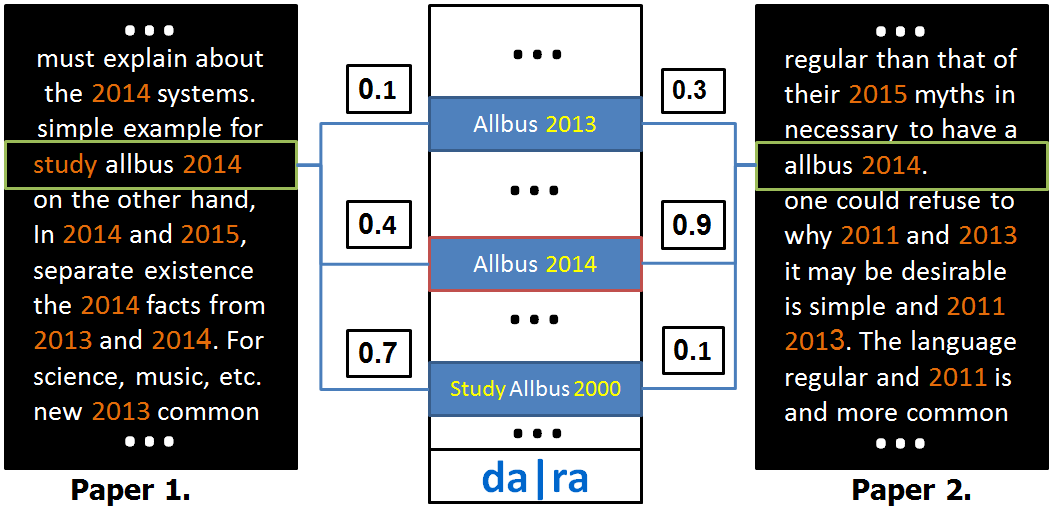
\includegraphics[width=4.5 in]{ToyExamplE.PNG} 
	\caption{A model example of cosine similarity, where tf-idf is computed over phrases in two papers.(The numbers are not from a real example)}
	\label{fig:similarity-example}
\end{figure}

In paper~1, \enquote{2014} repeats many times, whereas the word \enquote{study} occurs only once, which means the tf-idf assigns a high weight to \enquote{study} and a low weight to \enquote{2014}. When the query string is \enquote{study allbus 2014}, cosine similarity gives a higher rank to \enquote{Study Allbus 2000} than \enquote{Allbus 2014}.

To address this problem in a better way, our implementation employs some heuristics. This includes an algorithm that improves dataset rankings based on matching years in the candidate strings in both the paper and the datasets' titles. In the example, these heuristics improve the ranking of the \enquote{Allbus 2014} dataset when analyzing paper 1. 

%<newpart_34
Figure~\ref{fig:Overview_of_approach} shows an overview of our approach. Two steps labeled with \enquote{M} means they need human interactions. \enquote{M1} is about the preparation of lists of special features and \enquote{M2} is about making final decisions between candidates suggested by our approach.
%newpart_34>



\subsection{Step 4: Exposing the Results to the User, and Interactive Disambiguation}
\label{sec:expos-results-reus}	
the application of our approach supports two workflows through which an expert user can choose the best matches for the datasets cited by a paper from a set of candidates identified automatically. The sizes of these sets have been chosen according to the observations we made during the evaluation of the automated step, as explained in Section~\ref{sec:eval}.

One workflow works per reference: for each reference, five titles of candidate datasets are suggested to the user. While this workflow best supports the user in getting every reference right, it can be time consuming; each paper in our corpus contains 45 dataset references on average, but these \emph{references} only belong to an average number of 3 distinct \emph{datasets}.

The second alternative workflow takes advantage of this observation. It works per characteristic feature and suggests 6 titles of candidate datasets to the user for each feature (which may be common to multiple individual references in the paper). 

%<newpart_35
Finally, an RDF Graph will be exported as an output, which contains information about links identified between papers and datasets. To enable even further analysis of the links identified between papers and datasets, we export an RDF graph containing all candidate datasets identified in the latter workflow for each paper. For each candidate dataset, we represent the essential metadata of the dataset in RDF: DOI and title.

\begin{figure}[h]
	\centering
	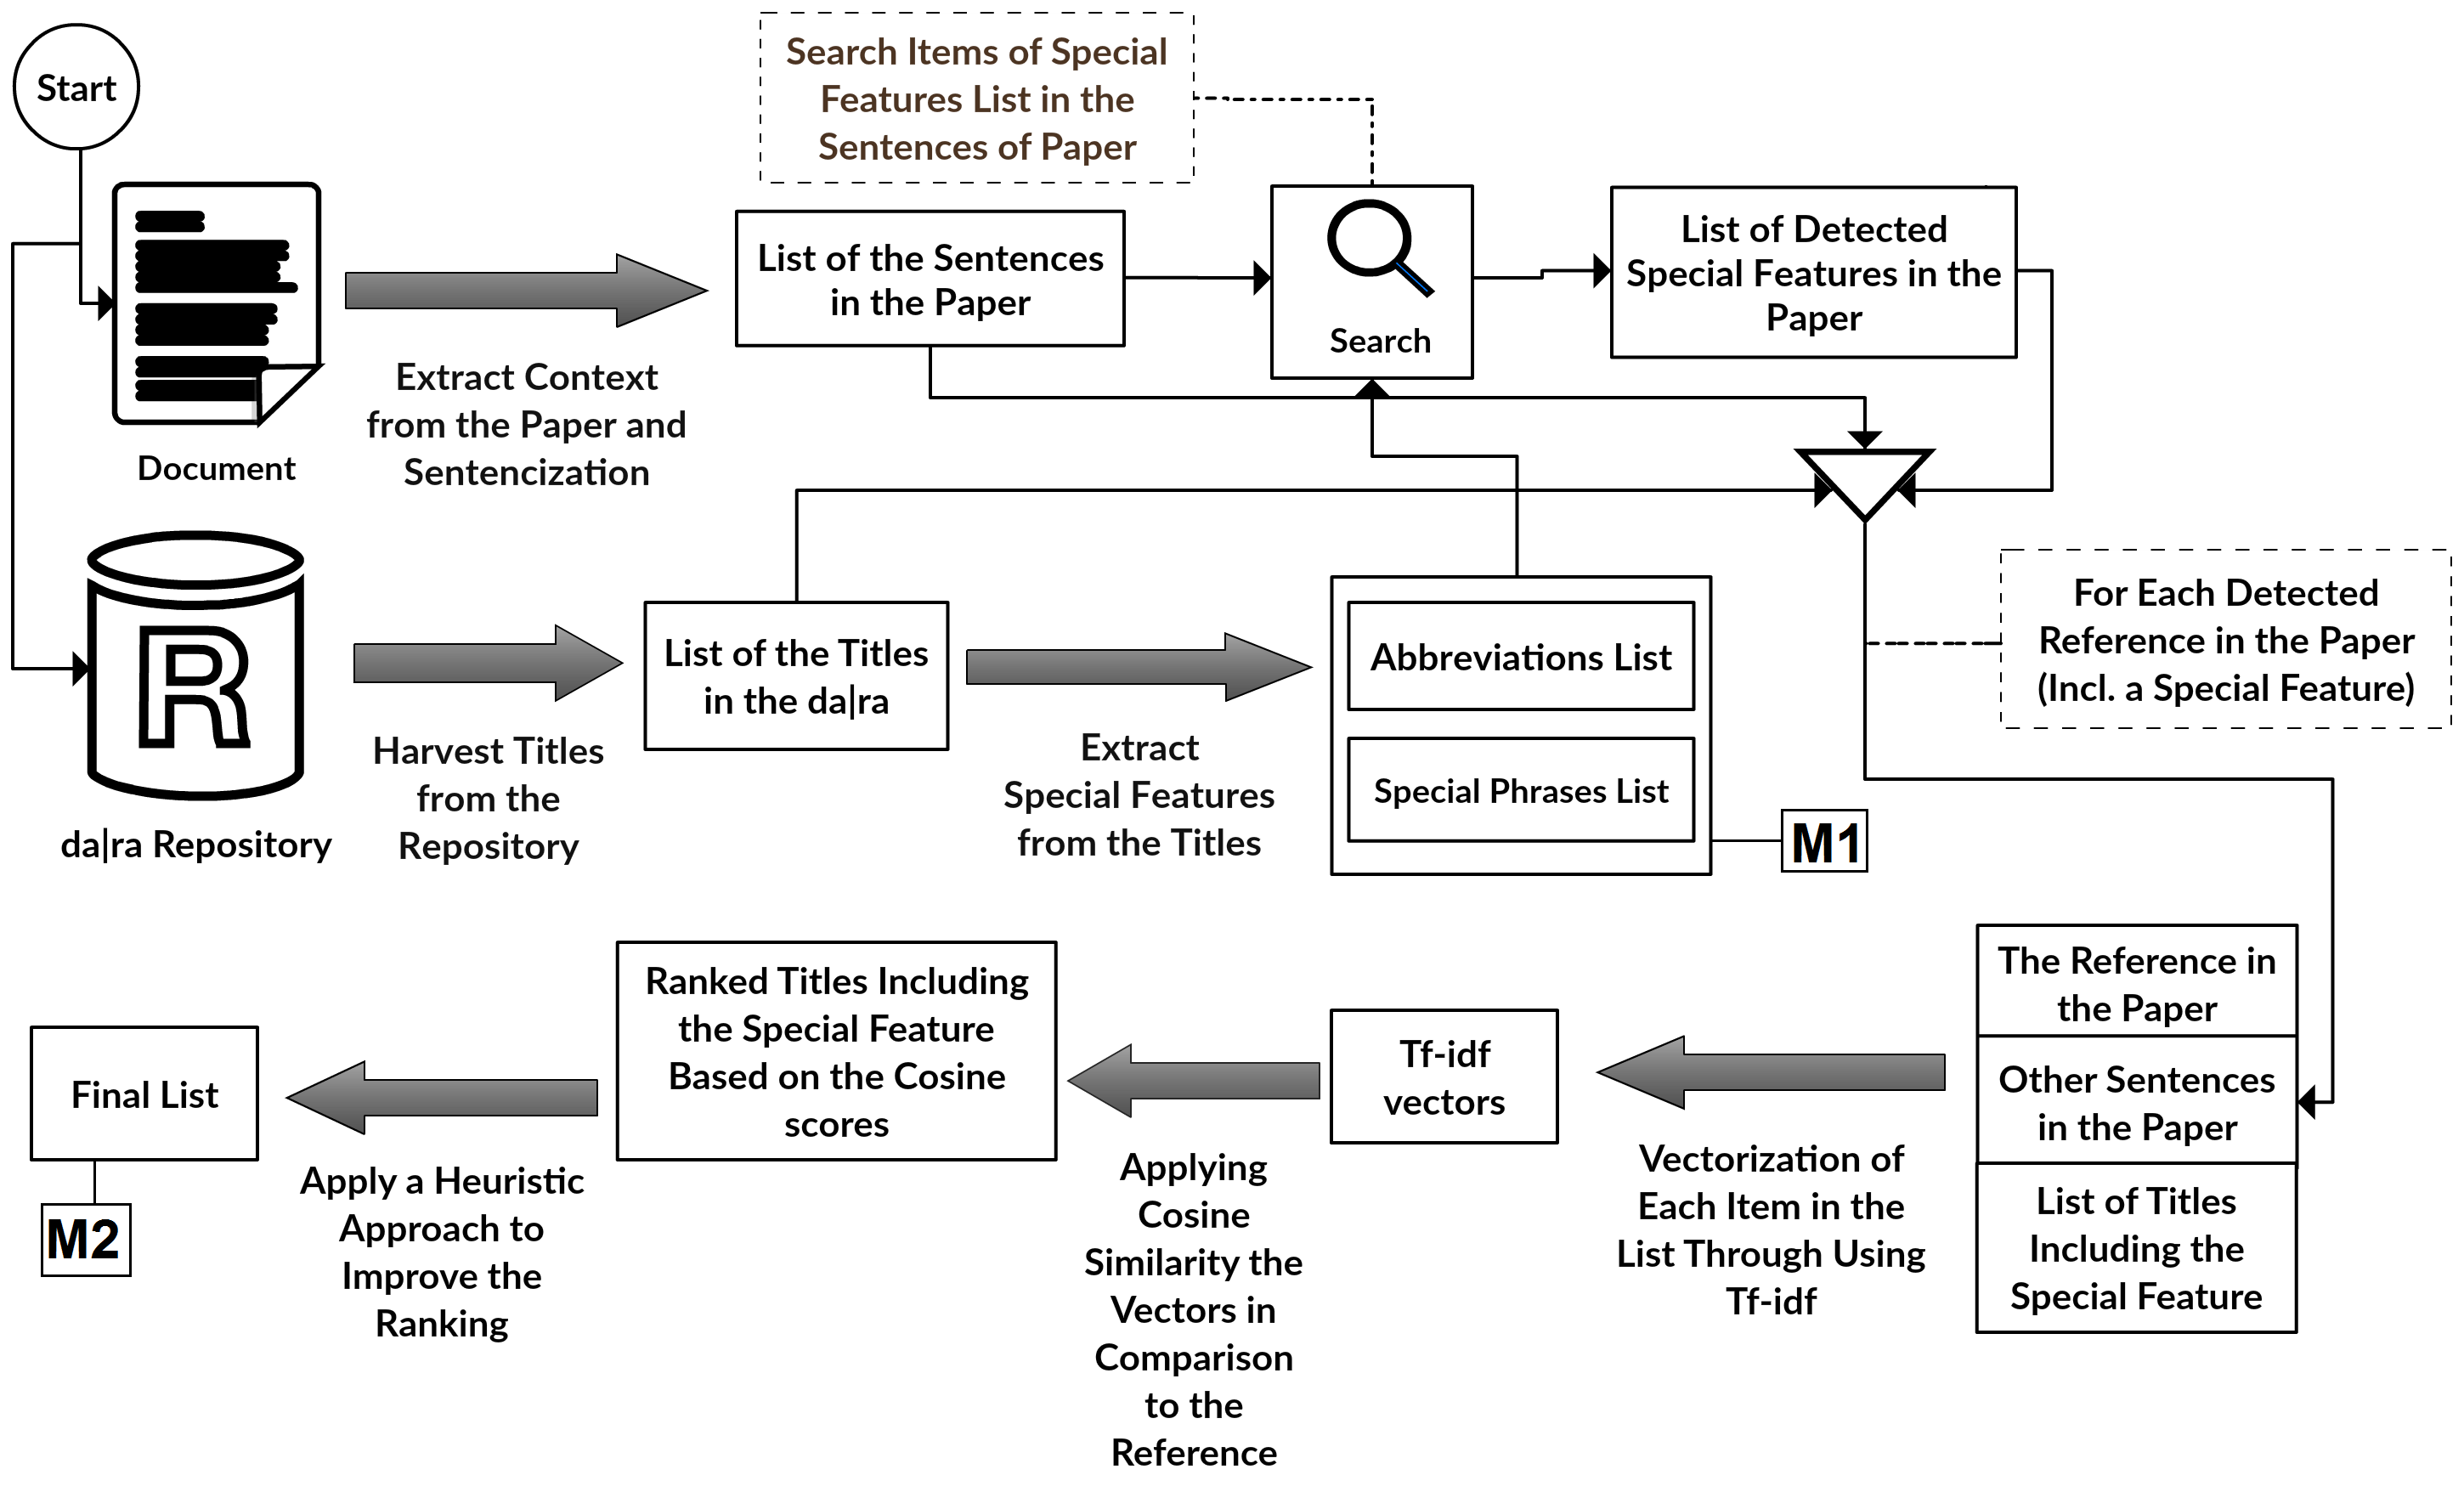
\includegraphics[height=3in]{Overwveiw_System.png}
	\caption{An overview of the approach.}
	\label{fig:Overview_of_approach}
\end{figure}
%newpart_35>

\section{Evaluation}
\label{sec:eval}
 \label{sec:eval}
The calculation of evaluation metrics such as precision, recall, and F-measure require ground truth. We therefore selected a test corpus of 15 random papers from the 2013 and 2014 issues of the mda journal -- 6 in English and 9 in German. 
%<newpart_36
This test corpus includes 25 datasets without considering different versions of each dataset and you can find some more information about it in table~\ref{table:info-testcorpuse}.
%newpart_36>

A trained assessor from the InFoliS II project at GESIS reviewed all papers one by one and identified all references to datasets. Afterwards, the assessor attempted to discover at least one correct match in {\dara} for each detected reference, resulting in a lists of datasets per paper. These lists were used as a gold standard to compare with the results of our algorithm in order to examine differences and similarities.

%<newpart_37
\begin{table}[h!]
	\renewcommand{\arraystretch}{2}
	\centering
	\begin{tabular}{c c c c}
		\FL
		 & Max. & Min. & Avg.
		\ML
		Datasets in a Paper & 7 & 1 & 4
		\NN
		References to a Dataset & 147 & 1 & 12
		\LL
	\end{tabular}
	\caption{More information about our test corpus}
	\label{table:info-testcorpuse}
\end{table},
%newpart_37>

 
\subsection{Evaluation Process and Description}
We decided to divide our evaluation into two steps. The first step focuses on identifying dataset references in papers. Here, accuracy depends on the quality of the generated dictionaries of abbreviations and special phrases 
%<newpart_38
(the accuracy metrics used in the paper are explained in \ref{sec:precision-recall}).
%newpart_38>
 
Our algorithm searches these characteristic features (as explained in \ref{sec:detecting-ranking}) in the full texts; detection of any of these features may lead to the detection of a dataset reference (see row \enquote{Detection} in table~\ref{table:eval-results}). In this phase, if a characteristic feature is identified both in a paper and in the gold standard, it will be labeled as a true positive. If the feature is in the gold standard but not in our output, it will be labeled as a false negative, or as a false positive in the opposite case.
 
The second step of the evaluation is about the accuracy of matching detected references in papers with datasets titles in the {\dara} registry. This evaluation phase considers only true positives from the previous step. The lists of suggested matches for an item, both from the gold standard and from our output, are compared in this step. 
%<newpart_39
Since a dataset may occur on its own or be integrated together with other studies,
%newpart_39>
an item can have more than one true match (e.g. Allbus 2010 in ALLBUScompact 1980--2012). In this step, an item will be labeled as a false negative if none of the suggestions for the item in the gold standard appears in the output of our algorithm. The number of false positives and false negatives are equal in this step, since a missing corresponding match means the possession of false positives. True positives, false positives, and false negatives are counted and then used to compute precision and recall.

%<newpart_40 
The third row in table~\ref{table:eval-results} refers to the accuracy of two phases of the algorithm as one unit in order to find how well it works generally, and does not consider one specific section (i.e. identification or matching). In order to satisfy this purpose, we repeated the second phase of evaluation, but this time included all data from the first step and not only the true positives. If an item is identified as false positive in the first section of evaluation, it is labeled as such in the evaluation as well.   
 
\subsection{Evaluation Results}
\label{sec:evre}
The algorithm gains high precision in both the detection and matching phases, which means it has a much smaller number of wrong predictions. It also covers the majority of relevant data, which leads to high recall.
%newpart_40>
The results of evaluations that we calculated are shown in table~\ref{table:eval-results}.
 
\begin{table}[h!]
 	\renewcommand{\arraystretch}{2}
 	\centering
 	\begin{tabular}{c c c c}
 		\FL
 		Phase of Evaluation & Precision & Recall & F-measure
 		\ML
 		Detection & 0.91 & 0.77 & 0.84
 		\NN
 		Matching & 0.83 & 0.83 & 0.83
 		\NN
 		Detection+Matching & 0.76 & 0.64 & 0.7
 		\LL
 	\end{tabular}
 	\caption{Results of the Evaluation }
 	\label{table:eval-results}
\end{table}
 
Our observations in the second evaluation step confirm the choices of set size in the interactive disambiguation workflows. In the per-reference matching workflow (as mentioned in \ref{sec:expos-results-reus}), a ranked list of dataset titles is generated for each of the 45 dataset references (on average in our corpus) in a paper by employing a combination of cosine similarity and tf-idf. 
 
Our observation shows that the correct match among {\dara} dataset titles for each reference detected is in the top 5 items of the ranked list generated by combining cosine similarity and tf-idf for that reference. Therefore, we adjusted our implementation to only keep the top 5 items of each candidate list for further analysis, such as an expert user's interactive selection of \emph{the} right dataset for a reference.
 
The per-feature matching workflow (as mentioned in \ref{sec:expos-results-reus}) categorizes references by characteristic features. For example, in a paper that contains exactly three detected characteristic features -- \enquote{ALLBUS}, \enquote{PIAAC}, and \enquote{exit poll} -- each dataset reference relates to one of these three features. If we obtain for each such reference the list of top 5 matches as in the per-reference workflow and group these lists per category, we can count the number of occurrences of each dataset title per category. 
 
Now, looking at the dataset titles per category sorted by ascending number of occurrences, we observed that the correct matches for the datasets' references using a specific characteristic feature were always among the top 6 items.
 
\section{Conclusion and future work}
\label{sec:future}
We have presented an approach for identifying references to datasets in social sciences papers.
It works in real time and does not require any training dataset.
There are just some manual tasks in the approach such as initially cleaning the dictionary of abbreviations, or making final decisions among multiple candidates suggested for the datasets cited by the given paper.
We have achieved an F-measure of 0.84 for the detection task and an F-measure of 0.83 for finding correct matches for each reference in the gold standard.  
Although the {\dara} registry is large and it is growing fast, there are still many datasets that have not yet been registered there. 
This circumstance will adversely affect the task of detecting references to datasets in papers and matching them to items in {\dara}.
After the evaluation, our observations reveal that {\dara} could cover only 64 percent of datasets in our test corpus. 

Future work will focus on improving the accuracy of detecting references to the datasets supported so far, and on extending the coverage to all datasets.
Accuracy can be improved by better similarity metrics, e.g., taking into account synonyms and further metadata of datasets in addition to the title.
Other algorithms such as identifying the central dataset(s) on which a paper is based can improve the ranked list generated by similarity metrics.
The identification of central dataset(s) is possible after pairing a share of references of datasets in a given paper with titles in {\dara}, and then this identification affects the ranking of rest of the references. 

Coverage can be improved by 
taking into account further datasets, which are not registered in {\dara}.
One promising further source of datasets is OpenAIRE, the Open Access Infrastructure for Research in Europe, which so far covers more than 16,000 datasets from all domains inluding social science but is rapidly growing thanks to the increasing attention paid to open access publishing in the EU.
The OpenAIRE metadata can be consumed via OAI-PMH, or, in an even more straightforward way, as linked data (cf.\ our previous work, \citet{VahdatiEtAl:MappingResearchMetadata15}).
For each dataset reference in the paper, we will model the precise position of that reference, and the algorithm's confidence in each possible matching dataset.
In a mid-term perspective, solutions for identifying dataset references in papers that have been published already could be made redundant by a wider adoption of 
standards for properly citing datasets while authoring papers, and corresponding tool support for authors.

\paragraph{Acknowledgements}
This work has been funded by the DFG project “Opening Scholarly Communication in Social Sciences” 
(grant agreements SU 647/19-1 and AU 340/9-1), and by the European Commission under grant agreement 643410. 
We thank Katarina Boland from the InFoLiS II project (MA 5334/1-2) for helpful discussions and for generating the gold standard for our evaluation. 
%<newpart_41
This Paper is an extension for our previous work~\cite{ghavimi2016identifying}. The implementation code is available in OSCOSS repository (link: \url{github.com/OSCOSS/Dataset_Detcter/tree/master/src}). 
%newpart_42>
\bibliography{biblo}
\end{document}
